% MAGNET, the human-readable paper. Two columns, 8 pages + references + appendix. Every number traces to a table or
% a k* script of the exhaustive version (paper/main.tex, "the long version" below). Build: tectonic main.tex
\documentclass[10pt,twocolumn]{article}
\usepackage[a4paper,margin=18mm,columnsep=7mm]{geometry}
\usepackage[utf8]{inputenc}
\usepackage[T1]{fontenc}
\usepackage{lmodern}
\usepackage{amsmath,amssymb}
\usepackage{booktabs}
\usepackage{graphicx}
\usepackage{microtype}
\usepackage{xcolor}
\usepackage[hidelinks]{hyperref}
\usepackage[numbers,sort&compress]{natbib}
\usepackage{caption}
\captionsetup{font=small,labelfont=bf,skip=4pt}
\graphicspath{{figures/}{../figures/}}
\newcommand{\magnet}{\textsc{magnet}}
\newcommand{\knn}{15-NN}
\setlength{\parskip}{0pt}
\title{\magnet{}: a sampled pass for the global structure, a full-batch pass for the local one, and a label-free community post-process}
\author{Maixent Chenebaux\\ \small Reputation Squad \quad \texttt{mchenebaux@trickstr.ai}}
\date{}

\begin{document}
\maketitle

\begin{abstract}
Neighbour embeddings pay for local fidelity with global arrangement, and the other way round. \magnet{} separates
the two: a sampled stochastic pass with a decoupled, heavy-tailed attraction places the clusters, a full-batch
FFT pass with $t$-SNE's objective refines the neighbourhoods, and an optional post-process translates and
contracts the communities of the fuzzy graph to raise the agreement of pairwise distances without using labels.
On MNIST 70k the full-batch pass reaches Barnes--Hut $t$-SNE's neighbourhood preservation (0.349 against 0.350)
in 6~s against 186, and the sequence has the highest pairwise-distance Spearman of the neighbour embeddings
tested; the post-process lifts the full-batch layout's Spearman from 0.35 to 0.47 and its $k$-means ARI from 0.76
to 0.91 at a cost of 0.002 of \knn{}, and does the same to a Barnes--Hut layout. We also report what we learned
on the way: the attraction exponent that maximises local fidelity at 70k tears data sets below 15k points into
micro-clusters and must follow the sample size; FIt-SNE's unit interpolation box leaves a 3.5\% force error that
costs 0.004 of \knn{}; and on kNN graphs the modularity's null model is nearly a constant, which splits large
geometric communities and swallows small ones, a failure that a density-contrast merge repairs with a threshold
read off a uniform cloud. [RESULTS: to be completed after the matched control experiment.]
\end{abstract}

\section{Introduction}
A 2-D layout of a data set is asked to do two things that pull apart. Locally, the neighbours of a point should
stay its neighbours; globally, the distances between clusters should keep their order. $t$-SNE and UMAP buy the
first with the second \citep{vandermaaten2008tsne, mcinnes2018umap}; PCA does the opposite; PaCMAP and TriMap
\citep{wang2021pacmap, amid2019trimap} add mid-range terms to a single objective and land in between. The long
version of this work (the exhaustive document this paper summarises, with every experiment and negative result)
argues that the two are better served by two passes with two objectives, and ships the result as a library.

\paragraph{Contributions.} (1) A two-pass method: a sampled SGD pass with a decoupled attraction kernel for the
global arrangement, a full-batch FFT pass with $t$-SNE's objective for the local structure, in that order, with the
hand-over scale set by a virial identity (Sec.~\ref{sec:method}). (2) The attraction exponent as a robustness
dial, and its dependence on the sample size: the heavy tail that maximises \knn{} at 70k tears small data sets
(Sec.~\ref{sec:exponents}). (3) An accuracy audit of the FFT pass: the interpolation, not the FFT, is the floor
(Sec.~\ref{sec:fft}). (4) A label-free post-process, placement of the graph's communities by a sampled
distance-rank objective under an overlap guard, then contraction; and a diagnosis of why modularity fails on kNN
graphs with a density-contrast merge that fixes it (Sec.~\ref{sec:post}). (5) Audited benchmarks on four data
sets with five-seed tables, frozen references and a matched control in which every competitor receives the same
post-process (Sec.~\ref{sec:results}).

\section{Two objectives, two passes}\label{sec:method}
\paragraph{Graph.} Both passes share one fuzzy $k$-nearest-neighbour graph ($k = 15$, NN-descent, UMAP's
per-row bandwidths, symmetrised), 1.2~s on MNIST 70k in our implementation.

\paragraph{Sampled pass.} UMAP's negative-sampling SGD on the graph with two changes. The attraction kernel
$\phi_b(d) = 1 / (1 + a d^{2b})$ carries its own exponent $b$, separate from the repulsion's Cauchy tail
($b_r = 1$): the force on a neighbour is $\sim d^{2b-1}$, nearly constant at $b = 0.6$, which makes the pull a
robust, median-like reading of a point's neighbours instead of a mean dragged by the far ones (Sec.~\ref{sec:exponents}).
And a weak mid-range spring on a sample of pairs at intermediate input distance, which raises the pairwise Spearman
by 0.02--0.04 at unchanged \knn{}. The pass runs 100 epochs, lock-free across threads, from a spectral start:
4~s on MNIST 70k.

\paragraph{Full-batch pass.} $t$-SNE's Kullback--Leibler objective on the same fuzzy graph (no perplexity
calibration), the repulsion by FIt-SNE's interpolation \citep{linderman2019fitsne} with three points per box of
width 0.7 (Sec.~\ref{sec:fft}), momentum and gains as in openTSNE \citep{policar2019opentsne}. Alone
(\texttt{loss="tsne"}): 600 iterations with early exaggeration from a PCA start, 6~s on MNIST 70k. As the second
stage of the sequence (\texttt{loss="hybrid"}): 300 iterations without exaggeration from the sampled layout, which
is first brought to the scale the objective wants.

\paragraph{Hand-over scale.} Writing $u_{ij} = s^2 d_{ij}^2 / (1 + s^2 d_{ij}^2)$ for the layout dilated by $s$, the
derivative of the objective in $\log s$ is $2(\mathbb{E}_p[u] - \mathbb{E}_q[u])$, so at a stationary point the
$p$-weighted mean of $u$ over the edges equals its $q$-weighted mean over all pairs; both sides cost one FFT
evaluation. The stationary dilation of the sampled layout is where the full-batch pass starts; a smaller scale
collapses the arrangement, a larger one re-expands and loses it (Appendix~\ref{app:virial}).

\paragraph{Why two passes.} The sampled pass arranges the clusters (its Spearman is 0.41 on MNIST against 0.30
for UMAP and 0.33--0.35 for the $t$-SNEs) but keeps 0.19 of \knn{}; the full-batch pass keeps 0.35 but arranges
little (0.35). The sequence keeps the local score of the second (0.353) and most of the global score of the first
(0.45). The long version shows that the order matters (the full-batch pass refines a layout, it does not repair
one), that the gain is not specific to our start (UMAP's layout refined by the same pass reaches the same
\knn{}), and that the mid-range spring is fatal inside the full-batch pass. Fig.~\ref{fig:layouts} shows the six
layouts.

\begin{figure*}[t]
\centering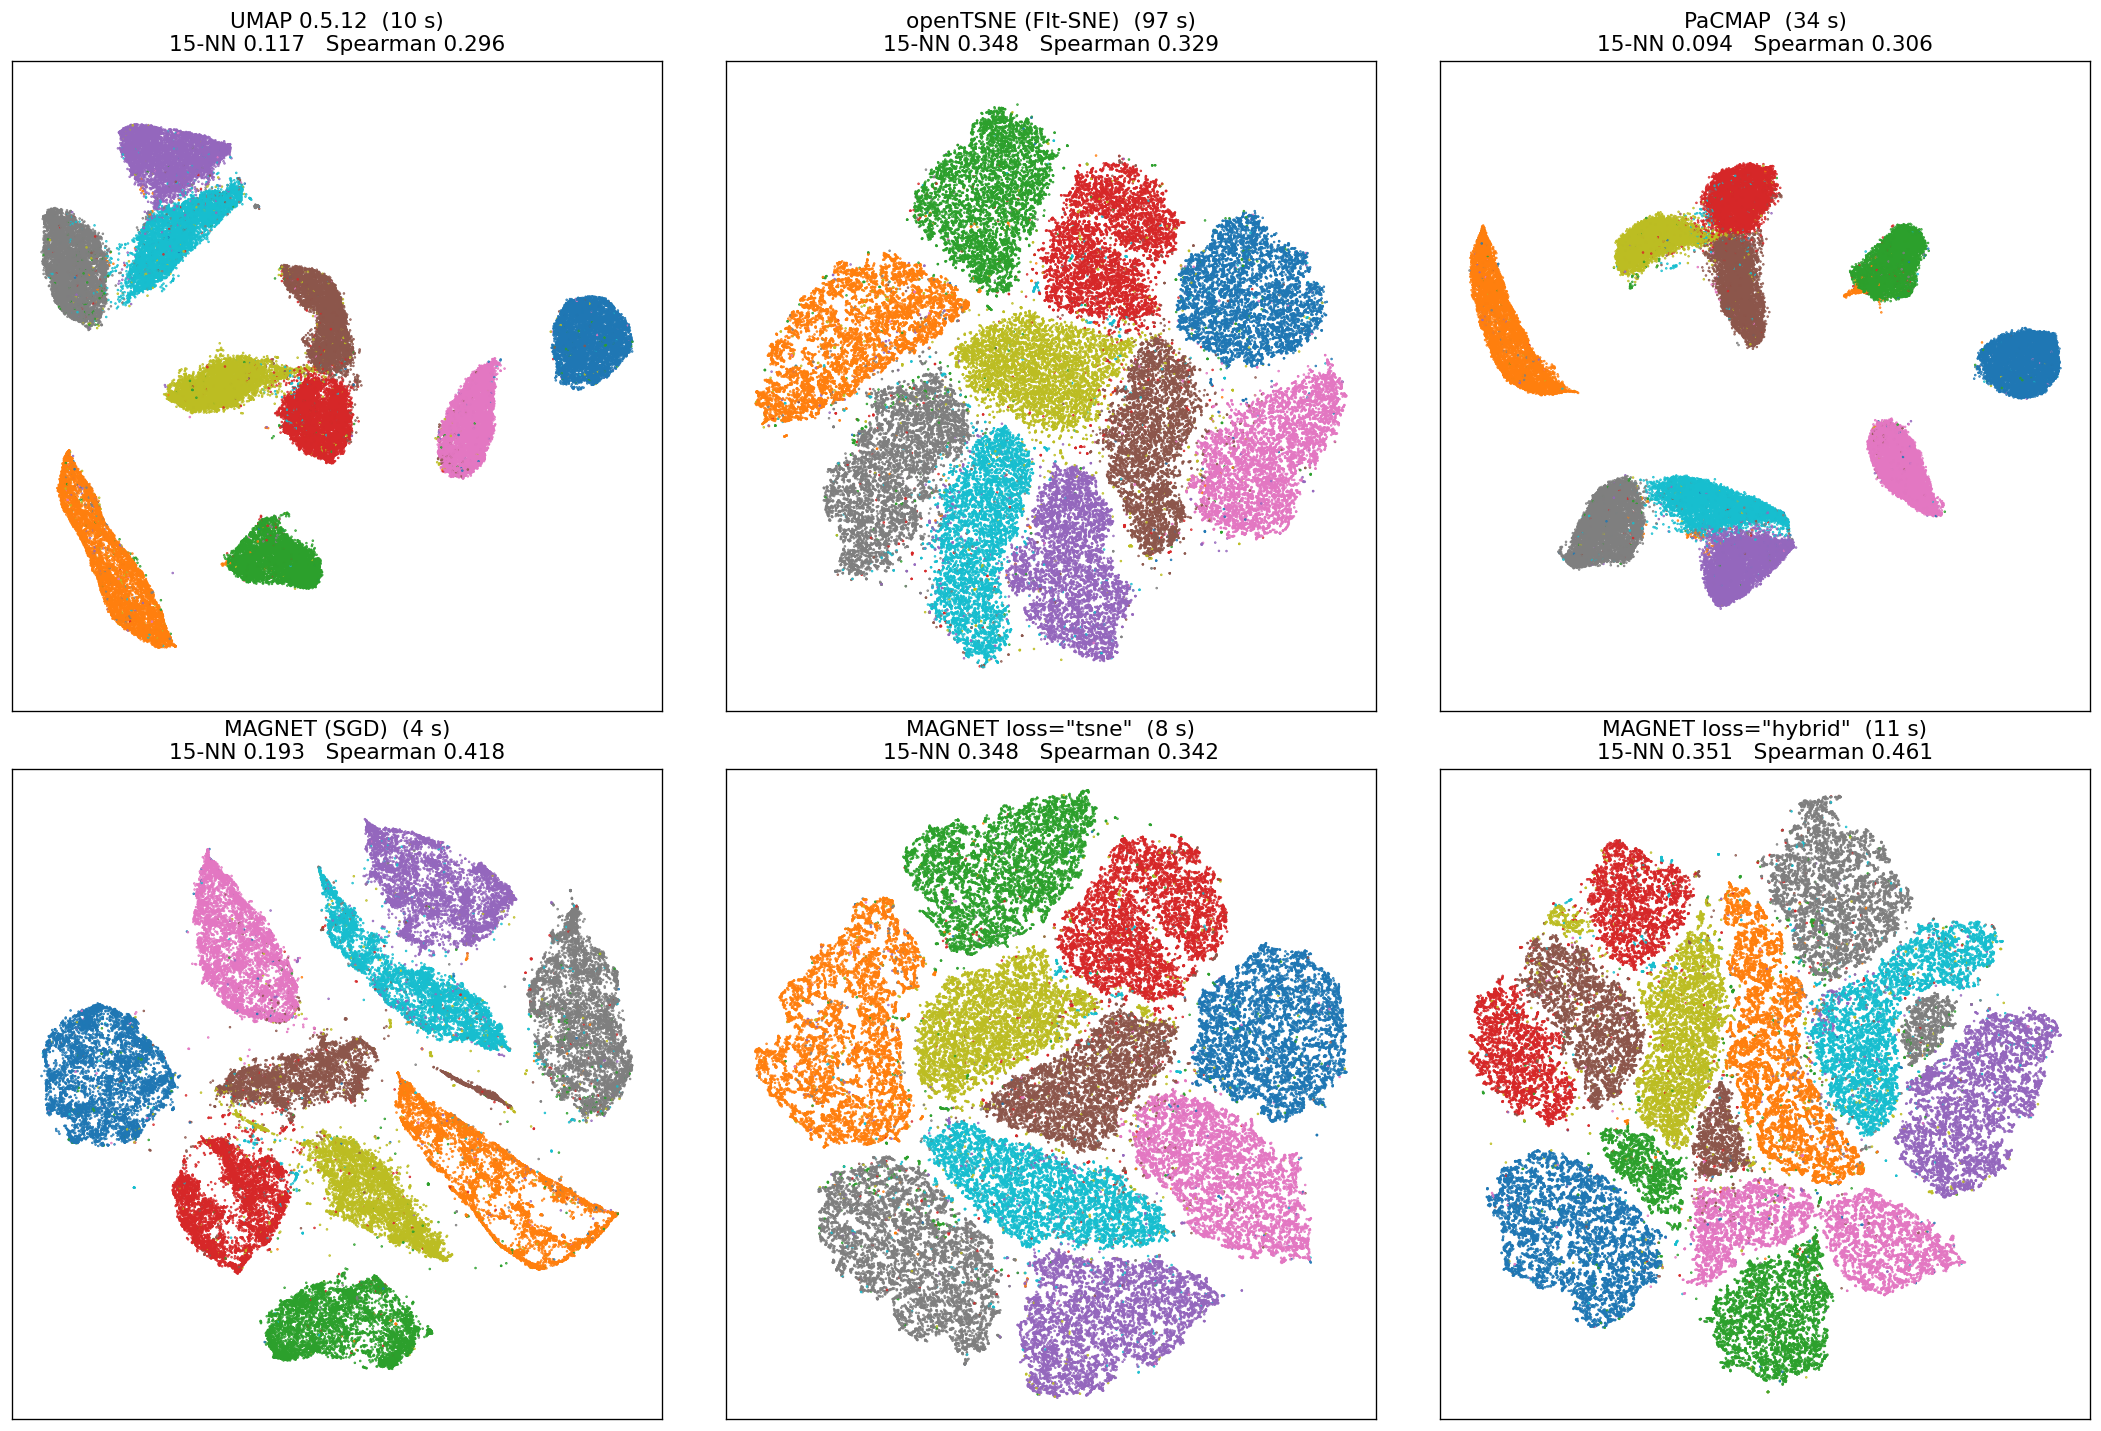
\includegraphics[width=\textwidth]{layouts_mnist.png}
\caption{MNIST 70k, same seed. Top: UMAP, openTSNE, PaCMAP. Bottom: \magnet{} sampled pass, full-batch pass,
sequence. Colours are the digit labels, not used by any method.}
\label{fig:layouts}
\end{figure*}

\section{The attraction exponent}\label{sec:exponents}
\paragraph{A robustness dial.} Sweeping $b$ with the repulsion fixed, \knn{} preservation peaks at $b = 0.5$ on
images and $0.6$--$0.7$ on text in one, two and three target dimensions alike (long version, Sec.~5). The reading
is Huber's: a point's neighbours in the input include contaminating far ones once the layout is crowded, and an
attraction whose force saturates at short range weights them like a median does, where the $L^2$-like force of
$b = 1$ weights them like a mean. An oracle that knows each point's contamination gains 5--10\% of \knn{} over
the fixed exponent; two label-free per-point versions reach a third of that.

\paragraph{It tears small data sets.} The same stiffness has a cost that only appears below some 15k points
(Fig.~\ref{fig:small_n}). Neighbours glue into tight clumps that only the redundancy of a dense graph knits
together; on MNIST subsamples HDBSCAN finds 56--78 density clusters in the layout at $n \le 10$k against 8 at
$n \ge 20$k, with 20--28\% of the points as noise, while UMAP finds 6--8 everywhere; USPS (7k): 60; phonemes (4.5k):
34. $b = 0.8$ holds them together at a \knn{} cost of 0.02--0.03 (USPS: 9 clusters, HDBSCAN ARI 0.79 against UMAP's
0.74 at a \knn{} of 0.337 against 0.316), and $b = 1$ collapses MNIST 70k into three clusters. Epochs, learning
rate, $k$, threads, the coupled kernel and the per-point exponents do not change this. The default therefore
follows $n$: $0.6$ at $n \ge 20$k, $0.8$ at $n \le 10$k, log-linear between. A label-free criterion makes the
same choices without $n$: raise $b$ from 0.6 until the density clusters of the layout agree with the graph's own
communities (Sec.~\ref{sec:post}) at an adjusted Rand index of 0.7; it picks 0.7 on USPS, 0.8 on MNIST 5k, 0.6 at
20k and above, and 0.7 on Fashion-MNIST, where the labels prefer 0.6 because its classes are not density clusters.
It is shipped as an option for clustering pipelines.

\begin{figure}[t]
\centering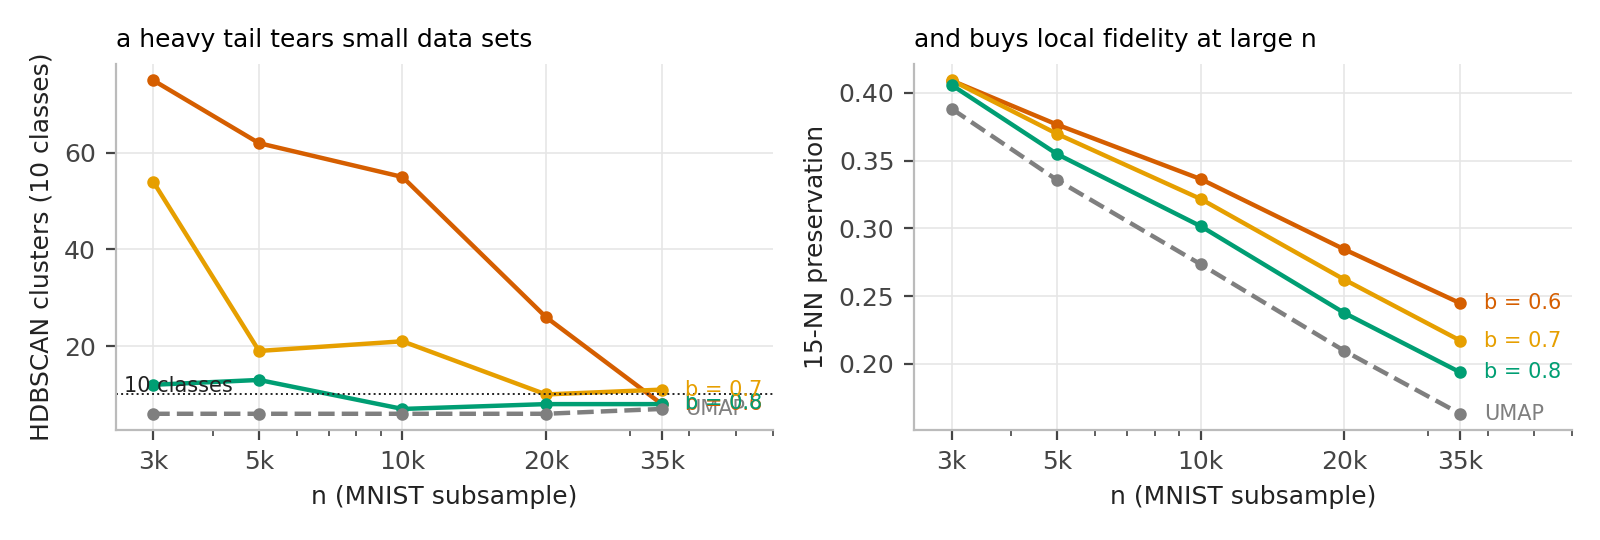
\includegraphics[width=\columnwidth]{fig_small_n.png}
\caption{MNIST subsamples, one run each. Left: density clusters found by HDBSCAN on the sampled-pass layout
(min cluster size $n/200$) for three attraction exponents, UMAP dashed. Right: \knn{} preservation. The heavy tail
is the best local reading at large $n$ and tears the layout at small $n$.}
\label{fig:small_n}
\end{figure}

\section{The full-batch pass is accurate to its grid}\label{sec:fft}
FIt-SNE interpolates the repulsive field on an equispaced grid, three Lagrange points per box of unit width in
layout units, and convolves by FFT. Against the exact all-pairs sum on MNIST's own layout the unit box leaves a
force error of 3.5\% RMS (1.2\% at width 0.7, 0.4\% at 0.5), and the error is what limits the result, not the
FFT: \knn{} rises monotonically as the box narrows, from 0.346 to 0.349--0.350 on MNIST (Barnes--Hut: 0.350) and
from 0.118 to 0.136 on Gaussian blobs, while the FFT cost grows as the inverse square of the width
(Fig.~\ref{fig:box}). Four or five interpolation points reach the same accuracy at a higher cost (the scatter
and gather touch 16--25 cells per point), dithering the grid does nothing, and the finer grid matters over the
whole post-exaggeration phase. Width 0.7 is the knee and the default, 15\% more time than the unit box. The
pass runs MNIST 70k in 6~s against 94 for openTSNE and 186 for scikit-learn's Barnes--Hut, both at their
defaults, with the same neighbourhood preservation as the second (long version, Table~2 and Appendix~D for the
timing protocol).

\begin{figure*}[t]
\centering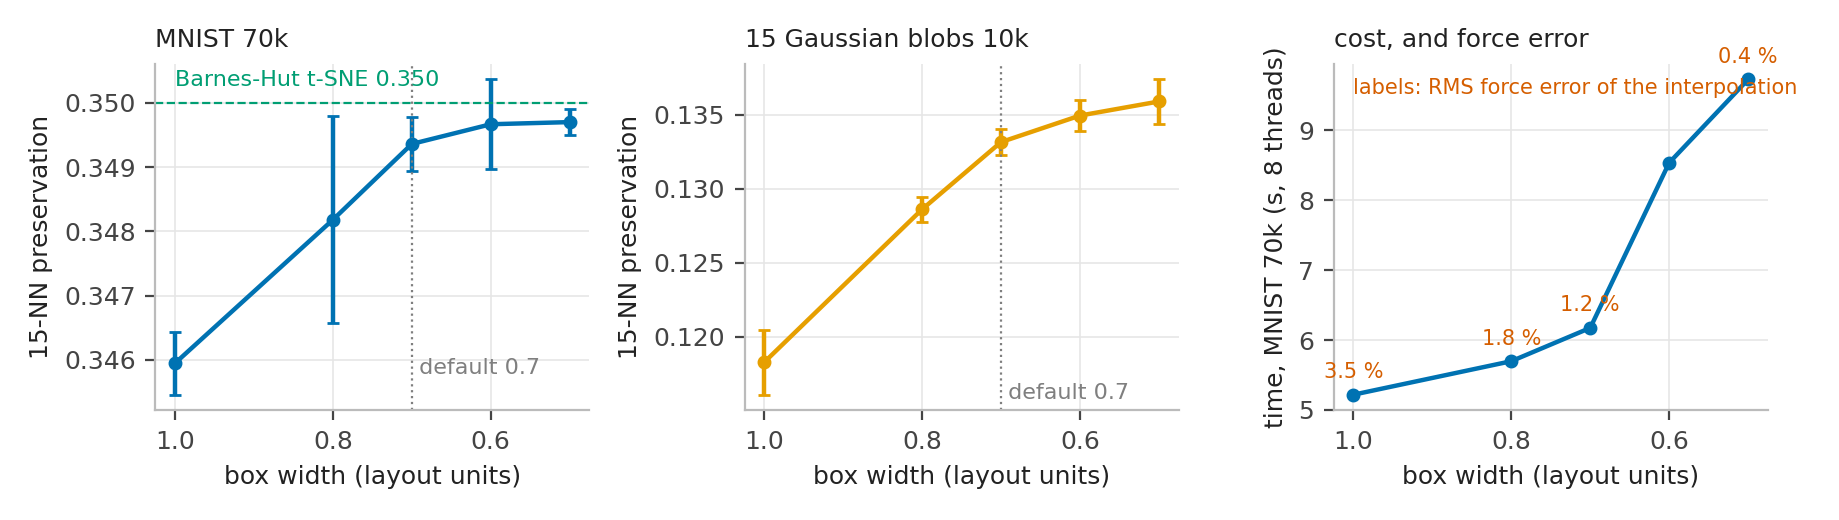
\includegraphics[width=\textwidth]{fig_box_width.png}
\caption{The interpolation box of the FFT pass. Left and middle: \knn{} preservation against the box width (mean
$\pm$ sd over 2--3 seeds). Right: time on MNIST 70k at 8 threads, labelled with the RMS force error of the
interpolation against the exact sum.}
\label{fig:box}
\end{figure*}

\section{Community placement and separation}\label{sec:post}
A $t$-SNE-like layout keeps neighbourhoods and spreads the classes apart, but its clusters are placed by the
history of the optimisation, not by the input distances: the pairwise-distance Spearman of the full-batch layout
is 0.35 on MNIST where PCA reaches 0.49. An optional post-process, label-free in execution, moves the clusters.

\paragraph{Communities.} The communities of the fuzzy graph, by Louvain. Two things had to be fixed. The random
visiting order made one run in three split a class on MNIST; visiting the nodes by decreasing strength is
deterministic and finds the ten classes on every graph tried. More fundamentally, the modularity's null model
expects a weight $\gamma k_i k_j / 2m$ between two nodes, and on a kNN graph every node has about the same strength,
so the null model is nearly a constant and the objective is the internal weight minus a penalty in (community
size)$^2$ (it coincides with the constant Potts model at the matched scale). A bisection of a uniform cloud of
$n_c$ points cuts $O(n_c^{1-1/d})$ edges while the penalty it saves grows as $n_c^2$, so large geometric communities
are split (the field-of-view limit of \citet{schaub2012markov}); a handful of boundary edges outweighs the tiny
size product of a small community, so it is swallowed (the resolution limit of \citet{fortunato2007resolution});
no resolution fixes both. What tells an artificial cut from a real boundary is the density across it. The
boundary nodes of $A$ towards $B$ (nodes of $A$ with an edge into $B$) send on average a share $f_{AB}$ of their
strength into $B$: across the thinnest cut of a uniform cloud that share is about 0.2 under our graph construction,
weakly dependent on the dimension and on $k$ (simulated, $d = 2$--$50$), and the Fiedler bisection of each MNIST
community gives 0.17--0.19; across a real class boundary at least one side reaches little
(Fig.~\ref{fig:interfaces}): $\min(f_{AB}, f_{BA})$ is 0.45--0.53 of the community's own cut share on MNIST's 25
real boundaries and 0.77--0.89 on its same-class splits. We run Louvain at a high resolution (no swallowing) and
merge interfaces while $\min(f_{AB}, f_{BA}) \ge 0.10$, half the no-contrast reference: the midpoint between no
contrast and a full gap. MNIST then has 10 communities on every graph and resolution tried; letter and covertype,
whose many small communities have asymmetric interfaces, are left almost untouched; Fashion-MNIST's touching
classes are merged into four, which is what the density says.

\begin{figure}[t]
\centering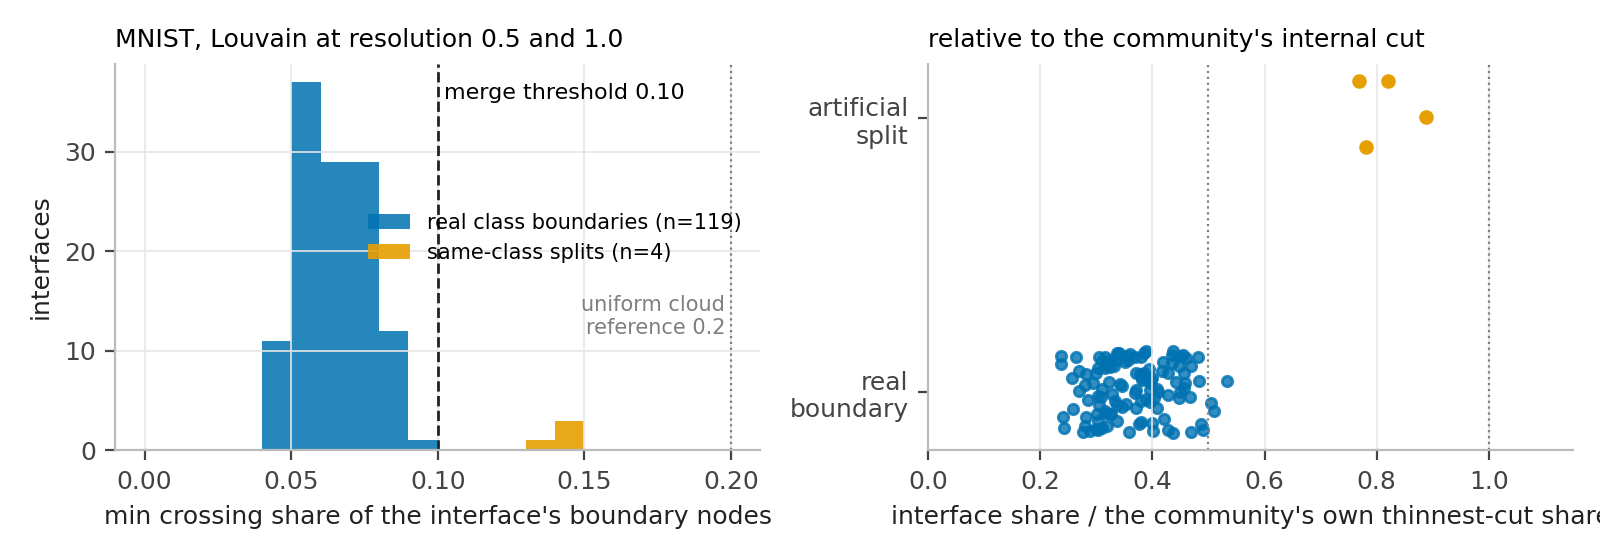
\includegraphics[width=\columnwidth]{fig_interfaces.png}
\caption{MNIST's fuzzy graph, communities of Louvain at resolutions 0.5 and 1.0 (over-partitioned). Left: the
smaller of the two crossing shares of each interface; the four same-class splits sit at 0.13--0.16, the 119 real
class boundaries below 0.10. Right: the same relative to each community's own thinnest internal cut.}
\label{fig:interfaces}
\end{figure}

\paragraph{Placement.} Each community with at least 1\% of the points, largest first, is translated as a rigid
body by the candidate (five radial scalings of its centroid offset and eight grid steps) that most raises the
Spearman correlation between the input and the layout distances of 500 sampled points, provided a guard holds:
the fraction of a 5000-point sample whose nearest sample point belongs to another community may not rise by more
than 0.002. Two sweeps, about 250 evaluations on the sample coordinates.

\paragraph{Separation.} Every community is then contracted about its centroid by $g = 0.7$. A similarity within
a community keeps the order of its distances; what changes is the arrangement and the gaps.

\paragraph{What it does.} On three seeds of MNIST's full-batch layout, with the search sample excluding the
benchmark's evaluation points: \knn{} / Spearman / $k$-means ARI 0.349 / 0.350 / 0.761 $\to$ 0.347 / 0.469 / 0.914
(run sd 0.000 / 0.001 / 0.004). Placement alone reaches Spearman 0.48 but lowers the ARI (the translations bring
communities closer), separation alone reaches ARI 0.92 at Spearman 0.33: the Spearman gain is the placement's, the
ARI gain the separation's. Two global metrics the step does not fit rise with it (triplet accuracy 0.627 $\to$
0.649, class-centroid Spearman 0.66 $\to$ 0.70). A Barnes--Hut layout receives the same gains (0.350 / 0.338 /
0.829 $\to$ 0.347 / 0.463 / 0.917): the step is method-agnostic, 1--2~s on 70k points, 6~s at 250k. Its settings
were chosen with the benchmark scores in view; it fits a sampled version of one reported metric; it can open
visual gaps at community boundaries of connected data. What did not work is in the long version (refining with
the KL after the step undoes it; a diffusion filter, soft borders and a placement without the guard lose \knn{};
a coarse two-community contraction was ``the zeros against the rest'').

\begin{figure*}[t]
\centering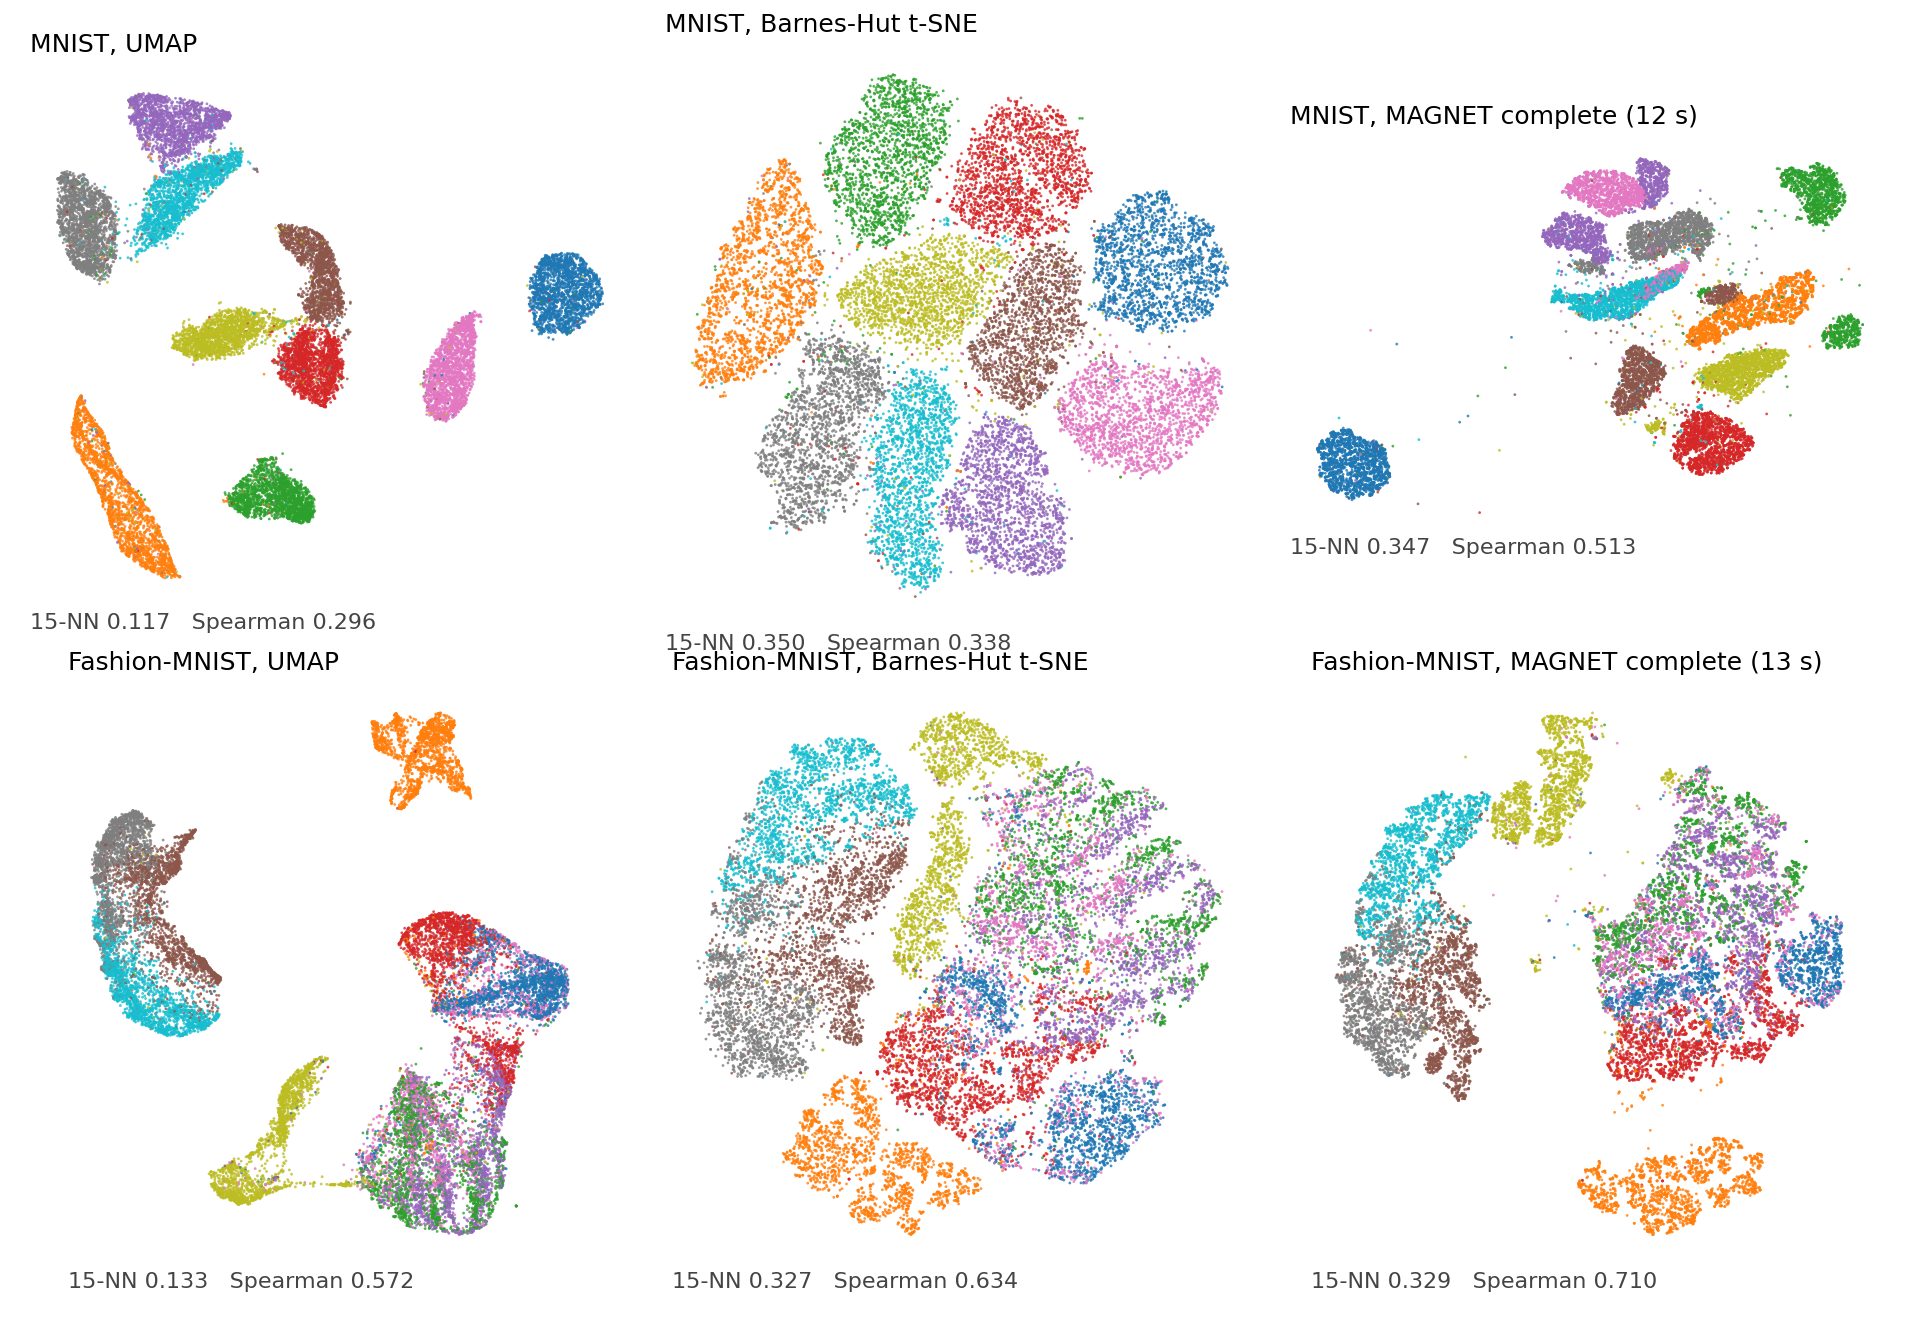
\includegraphics[width=\textwidth]{fig_pipeline.png}
\caption{The complete pipeline (sampled pass, full-batch pass, community placement and separation) next to UMAP
and Barnes--Hut $t$-SNE on MNIST and Fashion-MNIST 70k (20\,000 points shown, coloured by class, labels unused;
\knn{} preservation and pairwise-distance Spearman under each panel; single runs, seed 0). On MNIST the placement
sends the zeros far from the other digits because that is their input distance (class-centroid Spearman 0.66 $\to$
0.70); on Fashion-MNIST the step leaves four communities and opens gaps through connected data.}
\label{fig:pipeline}
\end{figure*}

\section{Results}\label{sec:results}
[TO FILL after k41: setup (data sets, metrics, frozen references, seeds, timing conditions); the five-seed table
of the decisive rows; the composite with one \magnet{} configuration in the main table and the rest in the
appendix; the matched post-process control; transfer to held-out data; time; what the panels do not show.]

\section{Limitations}
[TO FILL: hybrid $k$-means instability; Fashion's touching classes; small $n$ (phonemes); text; the HDBSCAN use
case is mixed outside MNIST; timings measured with a training job on the machine; the post-process targets one
reported metric; four data sets.]

\section{Conclusion}
[TO FILL.]

\bibliographystyle{plainnat}
\begin{thebibliography}{20}
\bibitem[van der Maaten and Hinton(2008)]{vandermaaten2008tsne} L. van der Maaten, G. Hinton. Visualizing data using $t$-SNE. JMLR 9, 2008.
\bibitem[McInnes et al.(2018)]{mcinnes2018umap} L. McInnes, J. Healy, J. Melville. UMAP: uniform manifold approximation and projection for dimension reduction. arXiv:1802.03426, 2018.
\bibitem[Wang et al.(2021)]{wang2021pacmap} Y. Wang, H. Huang, C. Rudin, Y. Shaposhnik. Understanding how dimension reduction tools work: an empirical approach to deciphering $t$-SNE, UMAP, TriMap, and PaCMAP for data visualization. JMLR 22, 2021.
\bibitem[Amid and Warmuth(2019)]{amid2019trimap} E. Amid, M. K. Warmuth. TriMap: large-scale dimensionality reduction using triplets. arXiv:1910.00204, 2019.
\bibitem[Linderman et al.(2019)]{linderman2019fitsne} G. C. Linderman, M. Rachh, J. G. Hoskins, S. Steinerberger, Y. Kluger. Fast interpolation-based $t$-SNE for improved visualization of single-cell RNA-seq data. Nature Methods 16, 2019.
\bibitem[Poli\v{c}ar et al.(2019)]{policar2019opentsne} P. G. Poli\v{c}ar, M. Stra\v{z}ar, B. Zupan. openTSNE: a modular Python library for $t$-SNE dimensionality reduction and embedding. bioRxiv, 2019.
\bibitem[Schaub et al.(2012)]{schaub2012markov} M. T. Schaub, J.-C. Delvenne, S. N. Yaliraki, M. Barahona. Markov dynamics as a zooming lens for multiscale community detection: non clique-like communities and the field-of-view limit. PLoS ONE 7(2), 2012.
\bibitem[Fortunato and Barth\'elemy(2007)]{fortunato2007resolution} S. Fortunato, M. Barth\'elemy. Resolution limit in community detection. PNAS 104(1), 2007.
\end{thebibliography}

\appendix
\section{The hand-over scale: a virial identity}\label{app:virial}
Let $Y$ have unit standard deviation and write $k_{ij} = (1 + s^2 d_{ij}^2)^{-1}$ for the kernel of the layout dilated by
$s$, $Z = \sum_{i \ne j} k_{ij}$ and $u_{ij} = s^2 d_{ij}^2 / (1 + s^2 d_{ij}^2)$. Differentiating the full-batch
objective $F(sY) = \sum p_{ij} \log p_{ij} - \sum p_{ij} \log k_{ij} + \log Z$ in $\log s$ gives
\[
\frac{\partial F(sY)}{\partial \log s} = 2\big(\mathbb{E}_p[u] - \mathbb{E}_q[u]\big)
= 2\Big(\textstyle\sum_{ij} p_{ij} u_{ij} - 1 + \sum_{ij} k_{ij}^2 / Z\Big),
\]
so at a stationary point the $p$-weighted mean of $d^2/(1+d^2)$ over the edges equals its $q$-weighted mean over all
pairs. Both sides cost one FFT evaluation ($\sum k_{ij}^2$ is the potential of the second FIt-SNE kernel with unit
charges). The stationary dilation $s^\ast$ of a start $Y_0$ is the root along the ray $sY_0$, confirmed as the minimum
of $F(sY_0)$ by a 13-point scan; it is conditional on the frozen shape of $Y_0$, not the equilibrium scale of the
jointly optimised layout. On MNIST 70k (long version, Table~3): $s^\ast = 85$--$102$ for our sampled starts, 10 for
PCA-2, about 120 for UMAP; the full-batch mode's own layout after 600 iterations is still far from its stationary
dilation (derivative $-0.05$ at four times its standard deviation), which is the radial component of the slow
expansion seen in the persistence runs. On MNIST subsamples $s^\ast$ grows as $n^{0.42}$ (28 / 54 / 85 at 5k / 20k /
70k).

The identity diagnoses the radial pressure but does not pick the hand-over. Handed over at $s^\ast$ the stiff start
gives \knn{} / Spearman 0.349 / 0.460 against 0.350 / 0.450 at 31 and 0.357 / 0.458 at 62, at five times the cost of
31; PCA-2 at its $s^\ast = 10$ gives 0.319 / 0.343 against 0.318 / 0.399 at 31. The scale is a dial between local
repair and global retention; the value that best trades the two is above the stationary one for PCA and below it
for our starts. The shipped rule, $31 \sqrt{n / 70000}$, is a finite-budget reference set on 70k points. Started
from $t$-SNE's tiny initialisation instead, the pass re-expands and loses the arrangement (Spearman 0.29--0.39);
started from the sampled layout's own scale it loses it as well.

\section{Staged refinement}\label{app:staged}
\paragraph{What was tested in the hand-over} (MNIST 70k, one start; long version, Sec.~3.1). Scale 15 / 31 / 62 /
124 with 300 iterations: \knn{} 0.338 / 0.353 / 0.357 / 0.338, Spearman 0.395 / 0.413 / 0.424 / 0.427 for a start at
0.428, in 6 / 10 / 30 / 121~s (the FFT grid follows the extent). Early exaggeration separated from the scale: at
scale 31, 0.352 / 0.458 without and 0.346 / 0.462 with; at the tiny scale 0.333 / 0.417 and 0.295 / 0.359: the
operative condition is the scale, the exaggeration costs little at the matched scale and is dropped. A mid-range
spring inside the second stage is fatal (\knn{} 0.118 at stiffness 0.1, collapse at 0.5). Iterations 25 / 75 / 150 /
300 / 600: \knn{} 0.277 / 0.328 / 0.343 / 0.353 / 0.352. Learning rate and kernel degrees of freedom buy nothing.
The reverse order (full-batch, then sampled epochs) returns \knn{} to the sampled level. Inside one full-batch
objective, a mid-range spring, a constant far-field repulsion and late exaggeration each cost \knn{} before the
Spearman moves.

\paragraph{The first stage can be tuned for global structure alone.} Since the second stage rebuilds the
neighbourhoods, a stiffer mid-range term in the first stage costs nothing locally after the pass and keeps most
of its Spearman gain: at stiffness 0.5 the start alone scores 0.178 / 0.459 and the sequence 0.356 / 0.442; at 0.1,
0.193 / 0.418 and 0.356 / 0.414. Stiffness 0.5 is the shipped compromise.

\paragraph{Is the gain the staging or the start?} The same pass applied to seven starts (long version, Table~1):
every neighbour-embedding start lands at 0.352--0.356 of \knn{} on MNIST and 0.327--0.331 on Fashion-MNIST over
five runs, at or above the standalone full-batch mode; the Spearman moves by $-0.02$ to $+0.04$ and is
predominantly inherited from the start; a start without neighbourhoods is not repaired in 300 iterations (PCA-2
reaches 0.315, a random start 0.065). Given the same affinities, start, scale and schedule, openTSNE's optimiser
and ours give the same scores: the pass is the objective and the hand-over, not the implementation.

\paragraph{Persistence.} From the stiff start the Spearman drifts from 0.480 to 0.470 at 300 iterations, 0.462 at
600, 0.455 at 1200 and 0.446 at 3000, while \knn{} rises from 0.346 to 0.367, the layout expands (standard
deviation 31 to 55) and the objective is still decreasing: the 300-iteration pass is an early stop, the limiting
Spearman is unknown. Two constraints that hold the coarse geometry through 1000 iterations at a local cost
(frozen Laplacian coordinates, a coarse rest-length scaffold) are in the long version's Appendix~C.

\section{All \magnet{} configurations}\label{app:configs}
[TO FILL: the seven configurations with raw axes, both composites against the frozen references, and time.]
\end{document}
